%%%%%%%%%%%%%%%%%%%%%%%%%%%%%%%%%%%%%%%%%%%%%%%%%%%%%%%%%%%%%%%%%%%%%%%%%%%%%%%%
%2345678901234567890123456789012345678901234567890123456789012345678901234567890
%        1         2         3         4         5         6         7         8

\documentclass[letterpaper, 10 pt, conference]{ieeeconf}  
\usepackage[utf8]{inputenc}

%\documentclass[a4paper, 10pt, conference]{ieeeconf}      % Use this line for a4
                                                          % paper

\IEEEoverridecommandlockouts                              
\overrideIEEEmargins

\usepackage{graphics}
\usepackage{epsfig} 
\usepackage{mathptmx} 
\usepackage{times} 
\usepackage{amsmath}
\usepackage{amssymb}
\usepackage{fancyhdr}
\usepackage{hyperref}
\pagestyle{fancy}
\fancyhf{}

\title{\LARGE \bf
Comunicación MQTT ESP8266 NODEMCU
}

\author{Pilatasig Jorge$^{1}$, Socasi Bryan$^{2}$, Viera Khaterine$^{3}$, Yánez Danilo$^{4}$% <-this % stops a space
}




\begin{document}

\maketitle
\thispagestyle{empty}
\pagestyle{empty}
\fancyfoot[]{Universidad de las Fuerzas Armadas "ESPE"}
%%%%%%%%%%%%%%%%%%%%%%%%%%%%%%%%%%%%%%%%%%%%%%%%%%%%%%%%%%%%%%%%%%%%%%%%%%%%%%%%
\begin{abstract}

In this project we will base ourselves on understanding how the MQTT communication works through a ESP8266 NodeMCU device and a web server that allows this communication to be carried out.

\end{abstract}


%%%%%%%%%%%%%%%%%%%%%%%%%%%%%%%%%%%%%%%%%%%%%%%%%%%%%%%%%%%%%%%%%%%%%%%%%%%%%%%%
\section{INTRODUCCIÓN}

La tecnología esta en constante innovación por lo que se a hecho necesario que los dispositivos electrónicos de uso cotidiano se puedan comunicar globalmente mediante el uso de la red.

Por lo que la comunicación MQQTT ESP8266 NodeMCU, permite que las maquinas hablen entre si, teniendo en uno de los extremos un dispositivo capaz de capturar datos a través de sensores, información como la temperatura, presión, humedad, que se envía a través de la red de datos, para ser almacenados en un servidor.

Esto permite que el dispositivo tenga una comunicación punto a punto a una interacción mas sofisticada donde se establezcan verdaderos diálogos entre las maquinas. Este protocolo permite una comunicación bidireccional por lo que se puede recibir y enviar mensajes.

\section{CONCEPTOS}

\subsection{IoT}

Internet de las cosas (en ingles, Internet of Things), es un concepto que se refiere a la interconexión digital de objetos cotidianos con internet.

\subsection{Comunicacion MQTT}

Es un protocolo usado para la comunicación $machine-to-machine$ (M2M) en el internet de las cosas. Este protocolo esta orientado a la comunicación de sensores, debido a que consume muy poco ancho de banda y puede ser utilizado en la mayoría de dispositivos empotrados con pocos recursos.

\begin{center}
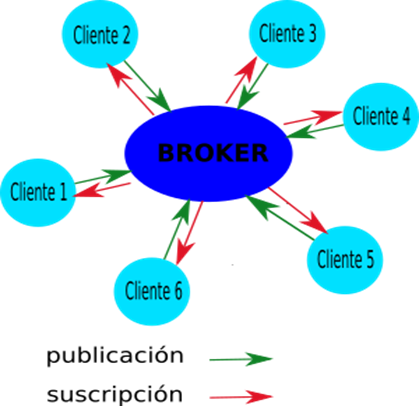
\includegraphics[scale=0.5]{Figura1.png}
\begin{scriptsize}\\ 
Fig 1. Gestiona la red de publicación y suscripción de mensaje.
\end{scriptsize}
\end{center}

\subsection{Arquitectura MQTT}

La comunicación se basa en unos "topics" (temas), cuando el cliente publica el mensaje, los emisores y receptores deben estar estar suscritos a el "topic" que el cliente registro. Esta comunicación puede ser de uno a uno, o de uno a muchos. 

\subsection{ESP8266}

El ESP8266 es un chip Wi-Fi de bajo costo, que funciona mediente el protocolo TCP/IP. Incluye un microcontrolador para manejar dicho protocolo y el software necesario para la conexion 802.11.

\subsection{NodeMCU}

Es un proyecto Open-Source para el desarrollo de un modelo sencillo de integrar la IoT, para ello se desarrollan modelos de hardware y software que facilite el desarrollo de programas y aplicaciones basadas en Wi-Fi.

\section{ESP8266 NodeMCU}
%\begin{figure}
%    \centering
%    \includegraphics{}
%    \caption{}
%    \label{fig:Definicion de pines de la Tarjeta de desarrollo ESP8266 NodeMCU}
%\end{figure}%

\subsection{Información de los pines del ESP8266}

\begin{table}[h]
\caption{Pines Disponibles}
\begin{center}
\begin{tabular}{|c||c|}
\hline
Denominación en placa & GPIO\\
\hline
D0 & 16\\
\hline
D1 & 5\\
\hline
D2 & 4\\
\hline
D3 & 0\\
\hline
D4 & 2\\
\hline
D5 & 14\\
\hline
D6 & 12\\
\hline
D7 & 13\\
\hline
D8 & 15\\
\hline
RX & 3\\
\hline
TX & 1\\
\hline
\end{tabular}
\end{center}
\end{table}

\begin{center}
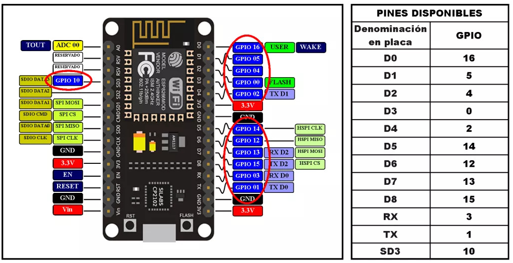
\includegraphics[scale=0.5]{Figura2.PNG}
\begin{scriptsize}\\ 
Fig 2. Diagrama de pines de la trageta de desarrollo
\end{scriptsize}
\end{center}


\subsection{Ventajas}

\begin{itemize}

\item Programación sencilla a traves de micro-USB
\item Alimentación a través del USB
\item Terminales (pines) para facilitar la conexion
\item LED y botón de reset integrados
\item La propia placa dispone de un regulador de alimentación, así como un chip USB-Serial para la comunicación del ESP8266 directamente desde el USB del ordenador
\item Facilidad de desarrollar aplicaciones de IoT debido a la gran comunidad y el gran numero de software compatible y librerías existentes para la programación del ESP8266

\end{itemize}

\section{ESTADO DEL ARTE}
\subsection{IoT}
En (Paroli, 2017) diseña e implementa un sistema de automatización para el hogar basado en el internet de las cosas industriales o IIoT. Este IIoT se desprende del internet de las cosas y pretende la conexión de objetos. Este proyecto cumplió con lo que es IzoT que es una plataforma abierta para la programación y desarrollo de redes de control industrial. Para su funcionamiento se han puesto controladores en diferentes puntos de la vivienda utilizada e interconectados a través de la red de datos de Ethernet estos funcionan como puntos de integración y control de diferentes periféricos. En este proyecto de utilizo el sistema operativo Linux y los servicios de control de Python.

\subsection{Pasarela de comunicación entre MQTT y DDs}
En la Universidad  de Sevilla (Manuel, 2015) desarrollo de una pasarela de comunicación entre DDS y MQTT, dos de los sistemas de mensajería utilizados en el área de M2M (machine-to-machine), son dos sistemas muy dispares, por lo que no toda la funcionalidad se puede traducir de uno a otro. El proyecto se centró en diseñar un intermediario DDS/MQTT que permita crear sistemas híbridos con clientes heterogéneos, es decir, un sistema a otro. 
La aplicación principal fue escrita en Java, utilizando RTI Connext y Eclipse Paho, su solución incluye una aplicación que le permite leer y escribir mensajes desde el lado MQTT: una aplicación de Rack en Ruby que proporciona una API que sigue el paradigma REST para ser utilizada a través de una mínima interfaz gráfica en HTML y JavaScript.

\subsection{Diagrama de Bloques}

\begin{center}
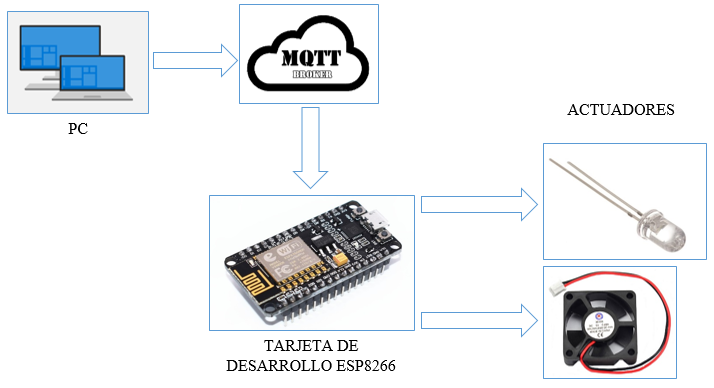
\includegraphics[scale=0.45]{Figura3.png}
\begin{scriptsize}\\ 

\end{scriptsize}
\end{center}

\section{EXPLICACIÓN DEL CÓDIGO FUENTEo}
En la primera parte del programa se especificará la librería que utilizaremos para comunicarnos y poder obtener las funciones de Cayenne. Además se definiraán las variables para concetarnos con la red, los requerimientos para realizar la comunicación MQTT y los pines que utilizaremos para la implementación del trabajo de investigación.

\begin{center}
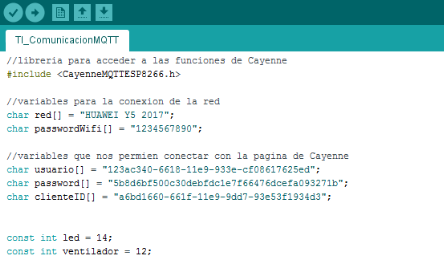
\includegraphics[scale=0.5]{Figura4.png}
\begin{scriptsize}\\ 
 
\end{scriptsize}
\end{center}

En la función setup() especificaremos que función cumplirán los pines de la tarjeta de desarrollo, si serán sensores INPUT o actuadores OUTPUT.
Luego iniciamos la comunicación con Cayenne myDevices con la función Cayenne.begin() que admite 5 parámetros. Los tres primeros son los datos para comunicarnos con Cayenne myDevices: usuario, password y clienteID.
Los dos siguientes son la configuración de la red WiFi: red y passwordWifi.

\begin{center}
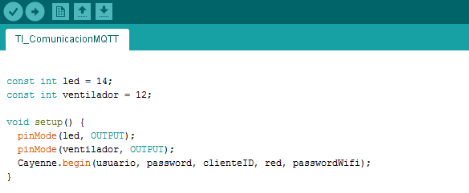
\includegraphics[scale=0.5]{Figura5.png}
\begin{scriptsize}\\ 
 
\end{scriptsize}
\end{center}

En función loop(). Lo primero es llamar a la función Cayenne.loop() donde se gestionará toda la comunicación con la plataforma en la nube.
A continuación en la siguiente función se procederá a leer el valor que tiene actualmente nuestro canal virtual 1 de Cayenne y se lo almacenará en la variable de tipo entero canalLed, para posteriormente con la función digitalWrite escribir en nuestro actuador la información que se está recibiendo en este instante por el canal virtual.
De igual manera se realiza con el canal virtual 2 en donde se controlará al ventilador.

\begin{center}
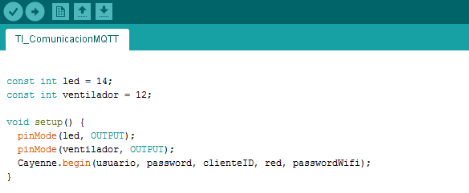
\includegraphics[scale=0.5]{Figura5.png}
\begin{scriptsize}\\ 
 
\end{scriptsize}
\end{center}

\section{CONCLUSIONES}
\begin{itemize}
    \item El protocolo de comunicación MQTT tiene un consumo realmente bajo, emplea muy pocos recursos para su funcionamiento por lo cual es muy empleado en la comunicación de sensores y actuadores que lo podemos aplicar al Internet de las cosas.
    \item Durante la realización del trabajo de investigación, hemos logrado implementar una de las tantas tecnologías existentes, de tal manera que nos sirva como ayuda para facilitar comunicaciones mediante software y programación.Durante la realización del trabajo de investigación, hemos logrado implementar una de las tantas tecnologías existentes, de tal manera que nos sirva como ayuda para facilitar comunicaciones mediante software y programación.
    \item El adquirir nuevos conocimientos en base a esta investigación nos ayuda a entender cómo se comunican los diferentes tipos de sensores y actuadores así como también como trabaja la cuarta revolución industrial.
    \item Logramos cumplir con cada uno de los objetivos, desarrollaando un circuto que nos permitio explicar el debido funcionamiento de cada uno de los componentes que lo constituye, a su vez logramos explicar cómo se desarrolla la comunicacionMQTT a traves de distintas aplicaciones web.
\end{itemize}


\addtolength{\textheight}{-12cm}   

\section{RECOMENDACIONES}
\begin{itemize}
    \item Siempre debemos comprobar que en el IDE de Arduino tengamos seleccionada la placa correcta, en nuestro caso la ESP82622 NodeMCU, ya que si se encuentra en cualquier otra, podemos averiar la tarjeta y además el servidor de Cayenne no lo reconocerá para realizar la conexión.
    \item Es mas complicada la programación haciendo un broker local como MQRR que utilizarlo en línea como Cayenne, por lo que para fines educativos es ideal usar Cayenne para entender de mejor manera el tema y acercarnos mas hacia el entendimiento loT (Internet of things).
    \item Conectar correctamente nuestros elementos a la placa del ESP8266 ya que aunque realicemos correctamente la programación y la configuración con el servidor, si los elementos como el LED o el ventilador se encuentran en los pines incorrectos o con la polarización indebida estos no podrán funcionar como esperamos.
\end{itemize}



\begin{thebibliography}{99}

\bibitem{c1} G. Alejandro, Plataforma domotica basadaen Raspberry Pi y el protocolo MQTT. Obtenido en: \url{http://wpd.ugr.es/~jorgenavarro/thesis/2017_TFG_AlejandroGarciaSoria.pdf}.
\bibitem{c2} M. Daniel, GEEKY THEORY. Obtenido en: \url{https://geekytheory.com/que-es-mqtt}
\bibitem{c3} Sitio web Electronics, Que es arduino. Obtenido de: \url{http://arduino.cl/que-es-arduino/}
\bibitem{c4} L. Jaime, Planta-Twittera. Obtenido de: \url{https://github.com/jaimelaborda/Planta-Twittera/wiki/1.-Introduccion-al-ESP8266-y-NodeMCU}
\bibitem{c5} L. Luis, Ingeniería, informática y diseño. Obtenido de: \url{https://www.luisllamas.es/esp8266-nodemcu/}
\bibitem{c6} M. Paroli, Diseño e implementación de un sistema de control integrado en el hogar basado en el concepto del internet de las cosas industriales para un departamento tipo suite. Obtenido de: \url{http://repositorio.espe.edu.ec/handle/21000/12917}

\end{thebibliography}

\end{document}
